\ESKDappendix{справочное}{Варианты использования системы\label{app:use_case}}

\begin{figure}[h]
\center{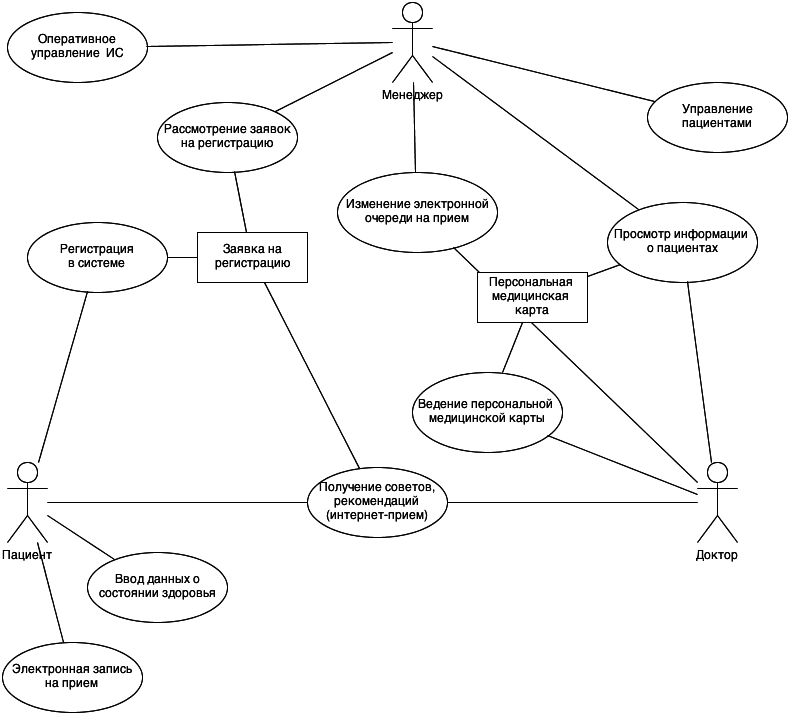
\includegraphics[width=1\linewidth,angle=90]{main_use_case.eps}}

% @startuml
% Менеджер -left-> (Оперативное управление ИС)
% Менеджер -> (Рассмотрение заявок на регистрацию)
% Менеджер -up-> (Изменение электронной очереди)
% Менеджер -down-> (Просмотр информации о пациентах)
% Менеджер -right-> (Управление пациентами)
% 
% Пациент -up-> (Регистрация в системе)
% Пациент -left-> (Электронная запись на прием)
% Пациент -down-> (Интернет-прием)
% Пациент -> (Ввод данных о состоянии здоровья)
% 
% Доктор -> (Просмотр информации о пациентах)
% Доктор -down-> (Ведение истории приемов)
% Доктор -down-> (Назначение лекарств)
% Доктор -down-> (Назначение диагнозов)
% Доктор -left-> (Интернет-прием)
% 
% note "Заявка на регистрацию" as bid
% (Регистрация в системе) .. bid
% bid .. (Рассмотрение заявок на регистрацию)
% @enduml

\end{figure}